\documentclass[11pt]{article}
\usepackage{geometry}                
\geometry{letterpaper}                   
\usepackage{graphicx}
\usepackage{subfigure}
\usepackage{subfig}
\usepackage{amssymb}
\usepackage{epstopdf}
%\usepackage{natbib}
\usepackage{amssymb, amsmath}
%\usepackage{cite}


\DeclareGraphicsRule{.tif}{png}{.png}{`convert #1 `dirname #1`/`basename #1 .tif`.png}

%\title{Robustness Analysis of Social Networks under Different Attack Models}
%\author{Name 1, Name 2, }
%\date{date} 

\begin{document}


\begin{document}
\thispagestyle{empty}


\begin{center}
%\includegraphics[width=5cm]{ETHlogo.eps}

\bigskip


\bigskip


\bigskip


\LARGE{ 	Lecture with Computer Exercises:\\ }
\LARGE{ Modelling and Simulating Social Systems with MATLAB\\}

\bigskip

\bigskip

\small{Project Report}\\

\bigskip

\bigskip

\bigskip

\bigskip


\begin{tabular}{|c|}
\hline
\\
\textbf{\LARGE{Robustness Analysis of Social Networks}}\\
\textbf{\LARGE{under Different Attack Models}}\\
\\
\hline
\end{tabular}
\bigskip

\bigskip

\bigskip

\LARGE{Ghosh, Partha \& Thapa, Manish Jung \& Acharya, Dinesh}



\bigskip

\bigskip

\bigskip

\bigskip

\bigskip

\bigskip

\bigskip

\bigskip

Zurich\\
May 2015\\

\end{center}



\newpage

%%%%%%%%%%%%%%%%%%%%%%%%%%%%%%%%%%%%%%%%%%%%%%%%%

\newpage
\section*{Agreement for free-download}
\bigskip


\bigskip

\large We hereby agree to make our source code for this project freely available for download from the web pages of the SOMS chair. Furthermore, we assure that all source code is written by ourselves and is not violating any copyright restrictions.

\begin{center}

\bigskip


\bigskip


\begin{tabular}{@{}p{1cm}@{}p{5cm}@{}@{}p{5cm}@{}@{}p{5cm}}
\begin{minipage}{3cm}

\end{minipage}
&
\begin{minipage}{6cm}
\vspace{2mm} \large Acharya, Dinesh

 \vspace{\baselineskip}

\end{minipage}
&
\begin{minipage}{6cm}

\large Ghosh, Partha

\end{minipage}
&
\begin{minipage}{6cm}

\large Thapa, Manish Jung

\end{minipage}
\end{tabular}


\end{center}
\newpage

%%%%%%%%%%%%%%%%%%%%%%%%%%%%%%%%%%%%%%%



% IMPORTANT
% you MUST include the ETH declaration of originality here; it is available for download on the course website or at http://www.ethz.ch/faculty/exams/plagiarism/index_EN; it can be printed as pdf and should be filled out in handwriting


%%%%%%%%%% Table of content %%%%%%%%%%%%%%%%%

\tableofcontents

\newpage

%%%%%%%%%%%%%%%%%%%%%%%%%%%%%%%%%%%%%%%

\section{Abstract}
Cascading failures 

\section{Individual contributions}

\section{Introduction and Motivations}

\subsection{Literature Review}
Most of the disease models categorise the given population into different categories and model the evolution of number of population in each of those categories with a set of differential equations. The popular susceptible infectious recovered (SIR) model is modelled by following set of differential equations:
\[ \frac{dS}{dt} = bN - \lambda S - dS,  \]
\[ \frac{dI}{dt} = \lambda S - gI - dI, \]
\[ \frac{dR}{dt} = gI - dR. \]

where $N = S + R + I$ is the total population size, $\lambda$ is the rate at which infectious individuals become infected, $g$ is the rate of recovery from infection, $d$ is the natural death rate and $b$ is the birth rate. The SIR models the diseases where there is no chance of infection once infected such as in the case of measles. Another popular model is susceptible-infectious-susceptible $SIS$ model which is given by following set of differential equations:
\[ \frac{dS}{dt} = gI - \lambda S,  \]
\[ \frac{dI}{dt} = \lambda S - gI. \]

SIS model is used to model diseases where there are high chances of repeated infections such as in the case of STDs like Chlamydia.

These standard models do not take into account the fact that pattern of interactions at individual level also play significant role in spread of disease. Standard Network Theoretic modelling of disease spread takes into account this factor by considering the network of individuals. Each individual is considered as a node and the possible interactions or contact between individuals is considered as a edge on the graph. The adjacency matrix $A$ is constructed such that $A_{ij} = 1$ if the disease can transfer from individual $i$ to individual $j$ and $0$ otherwise. The properties of the adjacency matrix can be studied to deduce about the structure of the network. To simulate disease spread in the network, different techniques has been used. One such model uses simple equation
\[ \text {rate of infection} = \tau \times n \] where n is number of infectious nodes in neighbourhood, $\tau$ is transmission rate. This has been discussed in more details on \cite{keeling}.

Similarly, the effect of structure of network on topology has been discussed in \cite{shirley}. There the authors use a probabilistic model to simulate the spread of disease in the network. At each step of simulation, a vertex was randomly picked. It then infects all of the neighbouring nodes with given probability of infection. The vertices remain infectious only for a certain latency period. After that, they are no more infectious and also immune to disease.

\subsection{Research Problem}
In this paper, we use a different differential equation to simulate the spread of disease in the network. We implement and discuss the cascading model by Helbing for disaster spread in terms of disease spread. Rather than spread of disease within a given population as in majority of related works, we look at spread of disease across cities in the whole world. So vertices represent cities rather than individuals in the given population.

With such differential equation, disease spreading in a social network (like cities or countries) will be investigated.  Our analysis is based on N-1 contingency. Meaning, it will be investigated whether or not the system is robust under single node failure; here failure implies node being infected by a disease. The goal of the project is to run N-1 contingency analysis with each of the nodes of the network attacked, for various kinds of real and artificial networks, and investigate which network is the most robust one. Various attack models will be used in the project- 

\begin{itemize}
\item Targeted attacks
\item Random attacks
\item Attack under certain probability distribution
\end{itemize}

 The number of nodes that fail, under the attack of initial node, will be registered. The same will be done for all the nodes in the network. The result will be averaged out and normalized with the system size and threshold parameter $\theta$ of the network. This will be done for several real and artificial networks, and the result compared to see the robustness of these networks under these attack models. Ultimately, the aim of this project is to construct a weighted robustness metric for social networks, which can very well be used across many disciplines like gas flow network, electricity grids, etc. given the dynamics of the cascading failure follows the differential equation. In addition, the evolution of cascading failure will also be investigated in the project. In other words, number of nodes that fail in each iteration also will be recorded, and the evolution of failing nodes displayed for each iteration.

\section{Description of the Model}

\section{Implementation}

\newpage
\section{Simulation Results and Discussion}
This paper gives a tool to quantify robustness of topologically different network against single random attack. The network is called N-1 robust if the damage it incurs is not significant under single node failure (infected). Our goal is to present a robustness metric tool to study whether or not a network is robust under arbitrary single node failure. To achieve this, a series of simulation experiments were performed using the disease spreading equation (X) under single node failures one-by-one for each of the network. In other words, the health of each node in network is recorded, and finally averaged for each iteration for each node-failure scenario. 

Figure 1 shows the different type of network studied in this paper. Small world network was studied for different distribution of node-degrees. These network was computer generated using Watts-Strogatz algorithm. Figure 2 shows the degree distribution for these networks. As the probability of edge rewiring among the nodes is increased, the network signifies random network, with non-uniform degree distribution. For $\beta=0$, the network is a ring lattice, with very small shortest path between any two nodes, and it represents the ideal small world. For larger $\beta$, the shortest path between any two nodes increases. Figure 3 shows the simulation result for these networks under the model in equation (X). As $\beta$ increases, the damage the network incurs decreases on average. This is particularly visible during the first iteration where the damage the network with smallest $\beta$ experiences is significantly higher than those with larger $\beta$. As can be observed, the evolution of average health reaches equilibrium after 16 iterations. 

\begin{figure}[!htb]
\centering
\subfigure[$\beta$=0]{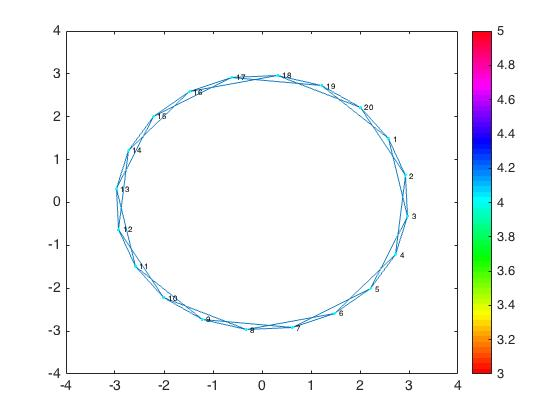
\includegraphics[width=0.49\columnwidth]{images/wattsa.jpg}}
\subfigure[$\beta$=0.15]{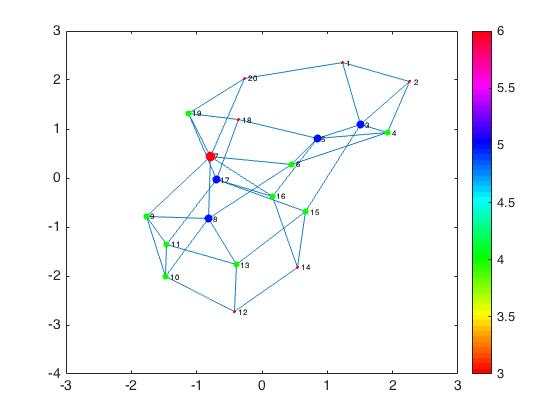
\includegraphics[width=0.49\columnwidth]{images/wattsb.jpg}}
\subfigure[$\beta$=0.5]{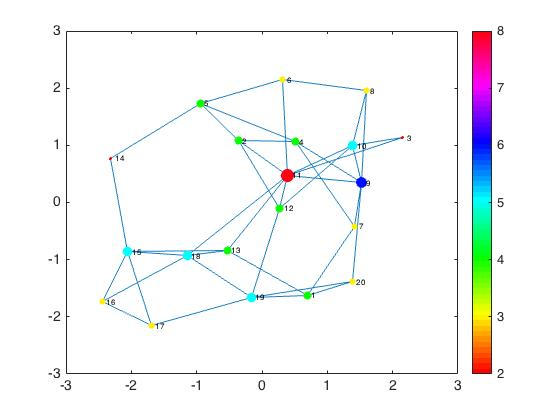
\includegraphics[width=0.49\columnwidth]{images/wattsc.jpg}}
\subfigure[$\beta$=1]{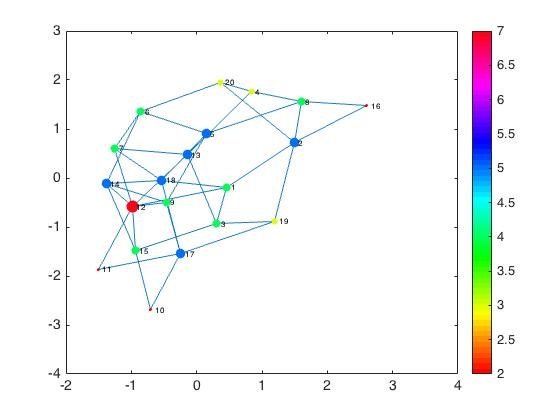
\includegraphics[width=0.49\columnwidth]{images/wattsd.jpg}}
\caption{Small world network constructed using Watts-Strogatz algorithm. The network size (N) and average node-degree (d) was fixed with N=20, and d=2, while the probability of rewiring ($\beta$) was gradually increased, making the network more and more random.}\label{fig:case-39-power-losses}
\end{figure}
\clearpage

\begin{figure}[!htb]
\centering
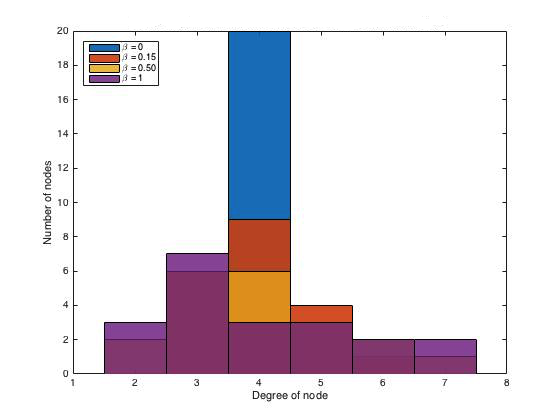
\includegraphics[width=0.69\columnwidth]{images/node_degree_distribution_20.jpg}
\caption{Node degree distribution for networks under investigation}
\end{figure}

Figure 4 shows the robustness metric under N-1 attach scenario for each of these networks. Each of this scatter point quantifies the robustness of the corresponding network; the smaller the average proportion infected per iteration the more robust is the network. The trend in the plot is quite clear. For smaller $\beta$, the less robust the network. 

\newpage

\begin{figure}[!htb]
\centering
\subfigure[beta0]{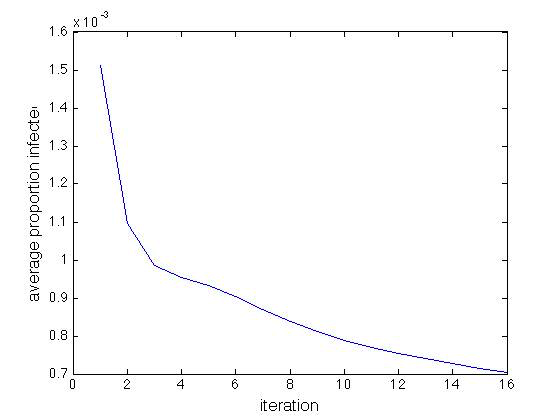
\includegraphics[width=0.49\columnwidth]{images/avgbetaa.jpg}}
\subfigure[beta0.15]{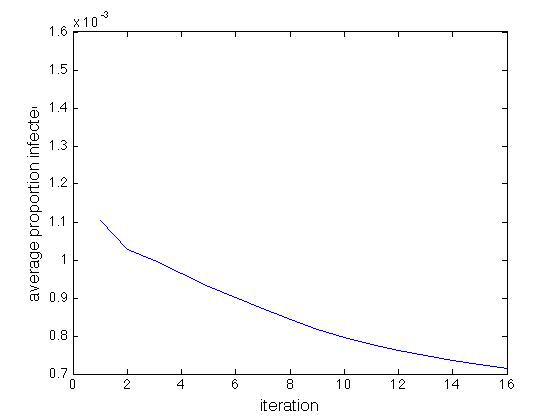
\includegraphics[width=0.49\columnwidth]{images/avgbetab.jpg}}
\subfigure[beta0.5]{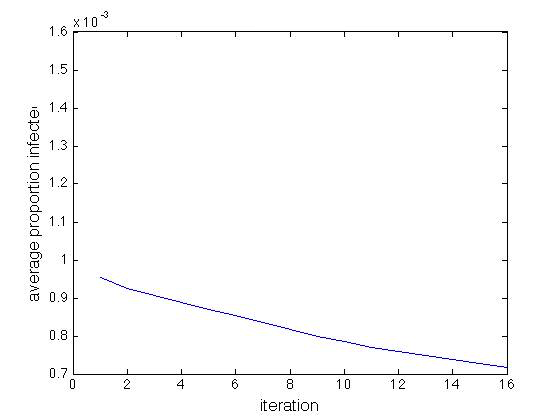
\includegraphics[width=0.49\columnwidth]{images/avgbetac.jpg}}
\subfigure[beta1]{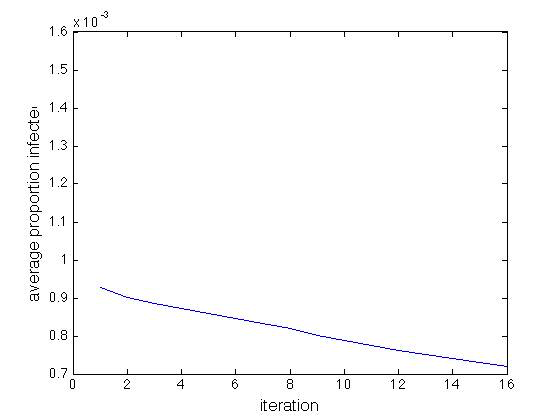
\includegraphics[width=0.49\columnwidth]{images/avgbetad.jpg}}
\caption{Power losses for case-39 with DC and AC power flow.}\label{fig:case-39-power-losses}
\end{figure}

\begin{figure}[!htb]
\centering
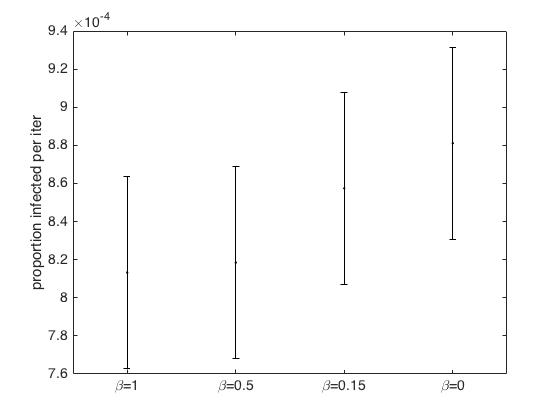
\includegraphics[width=0.60\columnwidth]{images/periter.jpg}
\caption{Node degree distribution for networks under investigation}
\end{figure}
\clearpage

\section{Summary and Outlook}
The more random the network, the more robust it is. Because for random network, the average path between any two nodes is 




\newpage
\begin{thebibliography}{9}
\bibitem{shirley} Shirley, Mark D.F. and Rushton, Steve P. \textit{ The impacts of network topology on disease spread }, Ecological Complexity, 2005.

\bibitem{helbing} Buzna, Lubos; Peters, Karsten; Ammoser, Hendrik;  Kuhnert, Christian and Helbing, Dirk.\textit{ Efficient Response to Cascading Disaster Spreading } .

\bibitem{keeling}
Keeling, Matt J. and Ken T.D. Eames. \textit{ Networks and Epidemic Models } Journal of the Royal Society Interface 2.4 (2005): 295–307. PMC. Web. 7 Dec. 2015.

\end{thebibliography}

\end{document}